\chapter{Using the icons}
The icons and logo images are stored on the control surfaces itself. You may simply connect to the surface using your webbrowser and type in the surface IP address (defaulti: 192.168.0.234). You will have to logon to the surface using your username/password (default: service/service). The main menu for this surface will be shown.

\vspace{5mm}

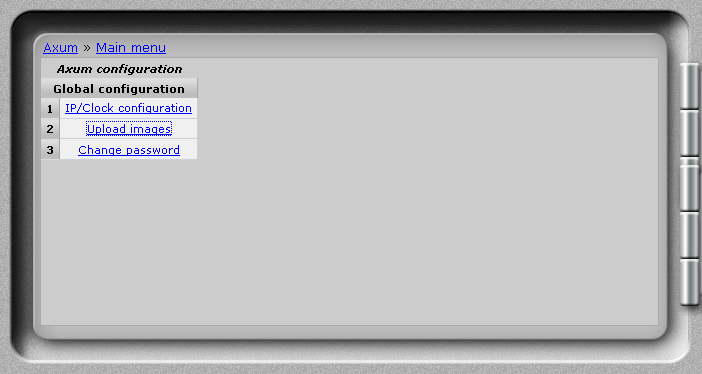
\includegraphics[width=13.5cm]{surfacemainmenu.png}

\vspace{5mm}

To upload images you can select menu item 2 'Upload images'

\pagebreak

\section{Upload}
Next you will see the upload page

\vspace{5mm}

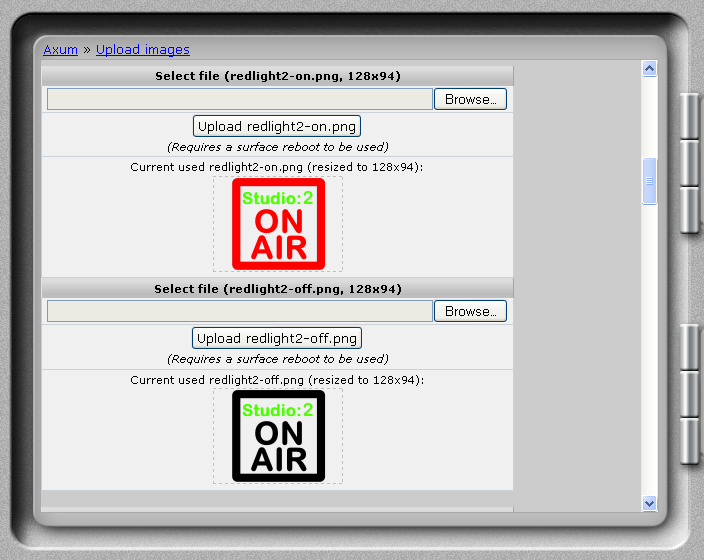
\includegraphics[width=13.5cm]{uploadpage.png}

\vspace{5mm}

You have to find the image you would like to replace and hit the corresponding browse button.

\vspace{5mm}

\pagebreak

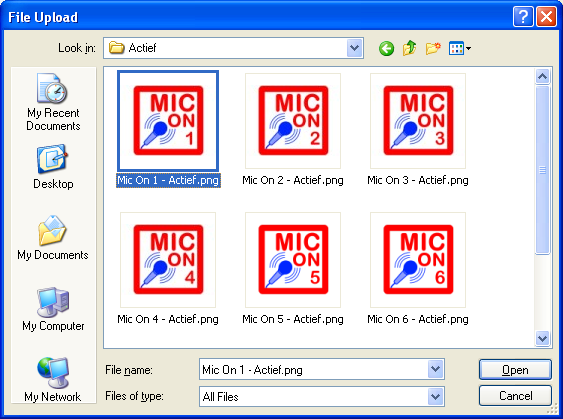
\includegraphics[width=13.5cm]{browseimage.png}

In this file box you have to select the PNG file you would like to upload. Eventually type '*.png' as filename to look for all PNG files in the current directory.

\pagebreak

\section{Configure functionality}
Once you have uploaded the custom icons you possibly would have to assign the corresponding functionality to the object. There for you have to browse to the webpage on the AXUM IO Rack (default 192.168.0.200).

\vspace{5mm}

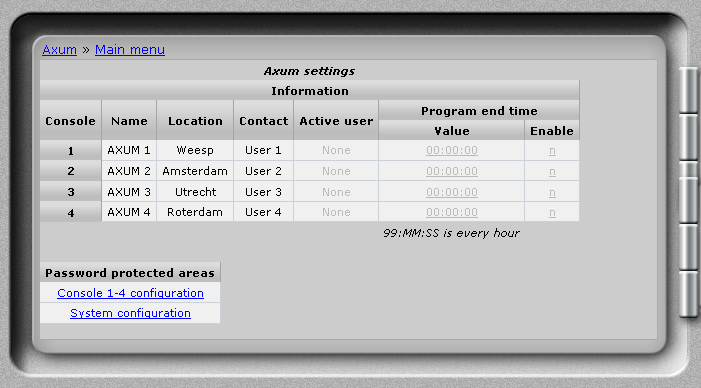
\includegraphics[width=13.5cm]{rackmainmenu.png}

\vspace{5mm}

You have to select 'Console 1-4 configuration' and log on with your username/password (default: service/service)

\vspace{5mm}

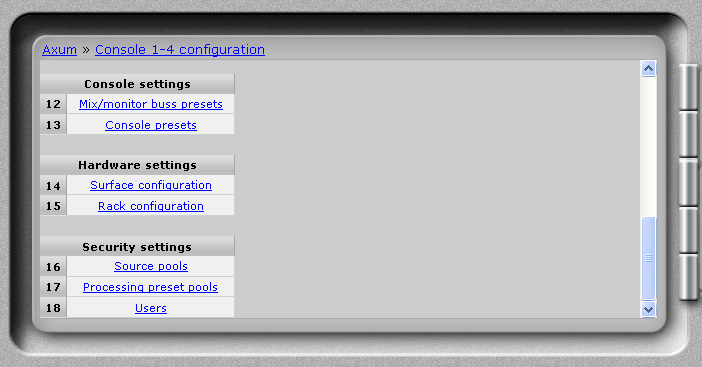
\includegraphics[width=13.5cm]{consoleconfig.png}

\vspace{5mm}

In th console configuration menu you select menu item 14, 'Surface configuration' 

\vspace{5mm}

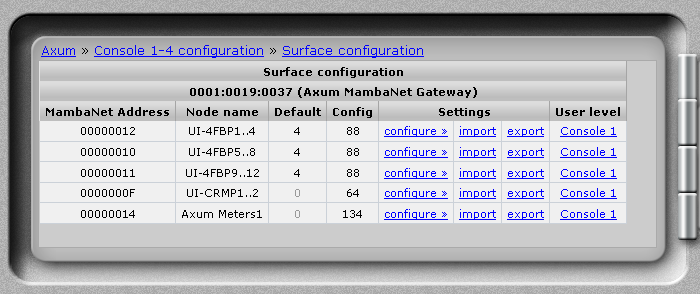
\includegraphics[width=13.5cm]{surfaceconfig.png}

\vspace{5mm}

Here you will see an overview of all surfaces that are found in your MambaNet-cloud and you may select the Axum-Meters node you would like to change its functionality.

\vspace{5mm}

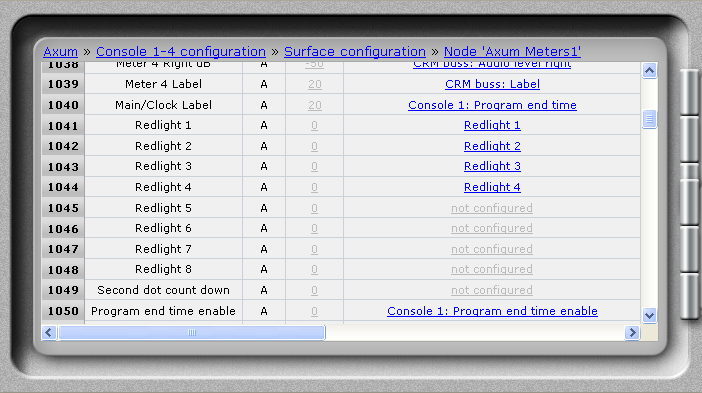
\includegraphics[width=13.5cm]{nodeconfig.png}

\vspace{5mm}

In the node configuration for the Axum-Meters node you have to scroll to the redlight objects where you can configure an function to use for this redlight.
There are many function that may be assigned to the GPIs, most interesting are:
\begin{itemize}
\item Global, redlight 1-8
\item Source, MIC, Module fader and on active
\item Source, Hybrid, Alert
\end{itemize}

But you are free to assign any function of the list to the 'redlight' objects.


